\chapter{動的計画法 - Dynamic programming}

\index{動的計画法 - dynamic programming}

\key{動的計画法 - Dynamic programming}とは
全探索の正しさと貪欲アルゴリズムの効率性を併せ持つ手法です。
動的計画法が適応できる場面とは、問題を独立に解くことのできる重複する部分問題に分割できる場面です。

動的計画法には大きく2つの使い方がある。

\begin{itemize}
\item
\key{最適解を見つける}:
できるだけ大きな解あるい小さな解を見つけたい。
\item
\key{解の数を数える}:
可能な解の総数を計算したい。
\end{itemize}

動的計画法の理解は、競技プログラマのキャリアのマイルストーンであるともいえます。
基本的な考え方は簡単ですが、様々な問題に対して動的計画法をどのように適用するかが課題となります。
この章では、出発点となる古典的な問題を紹介します。

\section{コイン問題 - Coin problem}

第6章ですでに見た問題ですが、再度注目しましょう。
この問題はコインの値の集合$\texttt{coins} = \{c_1,c_2,\ldots,c_k\}$
と目標金額$n$が与えられたとき、できるだけ少ないコインで合計$n$を形成することが課題でした。

第6章では、常に可能な限り大きなコインを選ぶ貪欲なアルゴリズムを使って問題を解きました。
貪欲アルゴリズムは、コインがユーロコインの場合などは有効ですが、
一般的な場合では必ずしも最適解が得られるとは限らないということも説明しました。

動的計画法を用いてどんなコインセットにも対応できるように効率的に問題を解決していきます。
動的計画法では総和を求めるために全探索のアルゴリズムと同様、すべての可能性を検討する再帰的な関数を用います。
この時にメモ化を使用して各部分問題の答えを一度だけ計算して効率的に動作させます。

\subsubsection{再帰的な式 - Recursive formulation}

動的計画法の考え方は、問題を再帰的な式として表現し、
より小さな部分問題の解から問題の解を計算できるようにしていきます。
コイン問題の場合、次のような再帰的な問題とします。
「和$x$を形成するのに必要な最小のコインはいくつですか?」

$\texttt{solve}(x)$を和xに必要なコインの最小枚数とすると、
関数の値はコインの値に依存します。
例えば,$\texttt{coins} = \{1,3,4\}$のとき,関数の最初の値は以下の通りです。

\[
\begin{array}{lcl}
\texttt{solve}(0) & = & 0 \\
\texttt{solve}(1) & = & 1 \\
\texttt{solve}(2) & = & 2 \\
\texttt{solve}(3) & = & 1 \\
\texttt{solve}(4) & = & 1 \\
\texttt{solve}(5) & = & 2 \\
\texttt{solve}(6) & = & 2 \\
\texttt{solve}(7) & = & 2 \\
\texttt{solve}(8) & = & 2 \\
\texttt{solve}(9) & = & 3 \\
\texttt{solve}(10) & = & 3 \\
\end{array}
\]

例えば、$\texttt{solve}(10)=3$は、和が10になるためには、
少なくとも3枚のコインが必要ということを意味します。
最適解は$3+3+4=10$です。

$\texttt{solve}$の本質的な特性は、
その値を再帰的に計算できることで、小さいコインの和から注目していきます。
例えば、上記のシナリオでは、最初のコインは1、3、4です。
最初にコイン1を選んだ場合、残っている課題は最小数のコインを用いて9を形成することとなります。
これは元の問題の下位問題となります。
コイン3、4についても同様です。
したがって,最小のコインの枚数を計算するには,次のような再帰的な公式を用いることができます。

\begin{equation*}
\begin{split}
\texttt{solve}(x) = \min( & \texttt{solve}(x-1)+1, \\
                           & \texttt{solve}(x-3)+1, \\
                           & \texttt{solve}(x-4)+1).
\end{split}
\end{equation*}
再帰の特殊な定式は$\texttt{solve}(0)=0$であり、
これは空の和を形成するためにコインは必要ないからです。

\[ \texttt{solve}(10) = \texttt{solve}(7)+1 = \texttt{solve}(4)+2 = \texttt{solve}(0)+3 = 3.\]

これで,$x$のための最小枚数を計算する一般的な再帰関数が準備できました。

\begin{equation*}
    \texttt{solve}(x) = \begin{cases}
               \infty               & x < 0\\
               0               & x = 0\\
               \min_{c \in \texttt{coins}} \texttt{solve}(x-c)+1 & x > 0 \\
           \end{cases}
\end{equation*}

$x<0$の場合、負の金額を形成することは不可能であるため値は$\infty$としましょう。
次に、$x = 0$のとき、値は$0$です。
なぜなら、負の金額を形成するためにコインは必要ためです。
最後に$x > 0$の場合,
変数$c$は最初のコインをどのように選ぶかについてすべての可能性を調べます。

問題を解く再帰の式が見つかれば、
C++で直接解を実装することができる(定数\texttt{INF}は無限大です)。

\begin{lstlisting}
int solve(int x) {
    if (x < 0) return INF;
    if (x == 0) return 0;
    int best = INF;
    for (auto c : coins) {
        best = min(best, solve(x-c)+1);
    }
    return best;
}
\end{lstlisting}

この関数は効率的とは言えません。なぜなら、和を構成する方法は指数関数的に増えるためです。
そこでメモ化と呼ばれる技術を使って、この関数を効率的にする方法を探ります。

\subsubsection{メモ化の利用 - Using memoization}

\index{メモ化 - memoization}

動的計画法の重要な考え方は\key{メモ化 - memoization}
を用いて再帰的な関数の値を効率的に計算することです。
つまり、一度計算した値はその関数用の構造に記憶します。
各パラメータに対して、関数の値は再帰的に計算して記録します。
次からは配列から直接値を参照します。

この例では配列を使用します
\begin{lstlisting}
bool ready[N];
int value[N];
\end{lstlisting}

\texttt{ready}[x]$は $\texttt{solve}(x) の値が計算されたかどうかを示し、
計算された$\texttt{value}[x]$にその値が格納される。
定数$N$は、必要な値がすべて配列に収まるように選ばれています。

この関数は次のように効率的に実装できるようになりました。
\begin{lstlisting}
int solve(int x) {
    if (x < 0) return INF;
    if (x == 0) return 0;
    if (ready[x]) return value[x];
    int best = INF;
    for (auto c : coins) {
        best = min(best, solve(x-c)+1);
    }
    value[x] = best;
    ready[x] = true;
    return best;
}
\end{lstlisting}

この関数は, 前と同様に $x < 0$ と $x = 0$ の基本ケースを処理します。
次に, $\texttt{ready}[x]$ を使って $\texttt{value}[x]$ に
$\texttt{solve}(x)$が既に格納されているかどうかをチェックして、
格納されていればそれを直接返します.
そうでない場合は、$\texttt{solve}(x)$の値を再帰的に計算し$\texttt{value}[x]$に格納します.

この関数は、各パラメータ$x$に対する答えを一度だけ再帰的に計算するため、効率的に動作します。
最初に$\texttt{solve}(x)$の値が$\texttt{value}[x]$に格納されるため、
$x$を指定して効率的に取り出すことができます.
このアルゴリズムの時間計算量は$n$を目標和$k$をコインの枚数とすると,$O(nk)$です。

なお,パラメータ $0 \ldots n$に対して$\texttt{solve}$ の全値を単純に計算するループを使って,
配列の値を反復的に構築しても良いです。
\begin{lstlisting}
value[0] = 0;
for (int x = 1; x <= n; x++) {
    value[x] = INF;
    for (auto c : coins) {
        if (x-c >= 0) {
            value[x] = min(value[x], value[x-c]+1);
        }
    }
}
\end{lstlisting}

多くの競技プログラマは、この実装の方が短く定数倍の計算量も低いので、
好んで使っています。
これ以降、私たちの例でも反復処理の実装を使用します。
しかし、動的計画法の解法は再帰的な関数で考える方が簡単な場合が多いというのは覚えておいてください。

\subsubsection{構築 - Constructing a solution}

しばしば、最適解の値だけではなく、どのように構成されるかの例を示すことの両方を求められることがあります。
これに応えるため、コインの問題では各金額について、
最適解の最初のコインを示す別の配列を宣言することができます。

\begin{lstlisting}
int first[N];
\end{lstlisting}
アルゴリズムを次のように改変しましょう。
\begin{lstlisting}
value[0] = 0;
for (int x = 1; x <= n; x++) {
    value[x] = INF;
    for (auto c : coins) {
        if (x-c >= 0 && value[x-c]+1 < value[x]) {
            value[x] = value[x-c]+1;
            first[x] = c;
        }
    }
}
\end{lstlisting}
以下のように和$n$の最適解に現れるコインを表示させることができます。
\begin{lstlisting}
while (n > 0) {
    cout << first[n] << "\n";
    n -= first[n];
}
\end{lstlisting}

\subsubsection{解のカウント - Counting the number of solutions}

ここで、コイン問題の別バージョンとして、
コインを用いて和$x$を生み出す方法 の総数を計算する問題を考えます。
たとえば,$\texttt{coins}=\{1,3,4\}$, $x=5$とすると
合計6通りあることになる.

\begin{multicols}{2}
\begin{itemize}
\item $1+1+1+1+1$
\item $1+1+3$
\item $1+3+1$
\item $3+1+1$
\item $1+4$
\item $4+1$
\end{itemize}
\end{multicols}

ここでも、再帰的に問題を解くことができます。
例えば、$\texttt{coins}=\{1,3,4\}$の場合、
$\texttt{solve}(5)=6$となり、再帰的な式は次のようになる。

\begin{equation*}
\begin{split}
\texttt{solve}(x) = & \texttt{solve}(x-1) + \\
                    & \texttt{solve}(x-3) + \\
                    & \texttt{solve}(x-4)  .
\end{split}
\end{equation*}

一般的な再帰関数は次のように示せます。
\begin{equation*}
    \texttt{solve}(x) = \begin{cases}
               0               & x < 0\\
               1               & x = 0\\
               \sum_{c \in \texttt{coins}} \texttt{solve}(x-c) & x > 0 \\
           \end{cases}
\end{equation*}

$x < 0$の場合、解が存在しないので値は0である。
$x = 0$の場合、空の和を形成する方法は1つしかないから値は1です。
それ以外の場合は$c$をコインとして、$\texttt{solve}(x-c)$ の形のすべての値の合計を計算する。

次のコードは、$0 \le x \le n$である時の
$\texttt{solve}(x)$の値
$\texttt{count}$を構築します。 

\begin{lstlisting}
count[0] = 1;
for (int x = 1; x <= n; x++) {
    for (auto c : coins) {
        if (x-c >= 0) {
            count[x] += count[x-c];
        }
    }
}
\end{lstlisting}

また、解の数が非常に多く、正確な数を計算する必要はないが、
例えば $m=10^9+7$ のように、$m$ のモジュロで答えを出せば十分なことがよくあります。
これは,すべての計算がモジュロ$m$で行われるようにコードを変更することで求められます。

\begin{lstlisting}
        count[x] %= m;
\end{lstlisting}
の後に次のようにします。
\begin{lstlisting}
        count[x] += count[x-c];
\end{lstlisting}

さて、ここまでで動的計画法の基本的な考え方はすべて説明しました。
動的計画法はいろいろな場面で使えるので、
これから動的計画法の可能性について、
さらに例を示す問題を見ていきましょう。

\section{最長増加部分列(LIS) - Longest increasing subsequence}

\index{最長増加部分列 - longest increasing subsequence}

\key{最長増加部分列(LIS) - longest increasing subsequence}
とは$n$個の要素を持つ配列の中で、最も長く増加する部分列を求める問題です。
言い換えると左から右へ向かう配列要素の最大長の並びで,並びの各要素は前の要素より大きくなるようなものです。
\begin{center}
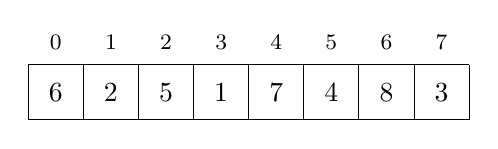
\begin{tikzpicture}[scale=0.7]
\draw (0,0) grid (8,1);
\node at (0.5,0.5) {$6$};
\node at (1.5,0.5) {$2$};
\node at (2.5,0.5) {$5$};
\node at (3.5,0.5) {$1$};
\node at (4.5,0.5) {$7$};
\node at (5.5,0.5) {$4$};
\node at (6.5,0.5) {$8$};
\node at (7.5,0.5) {$3$};

\footnotesize
\node at (0.5,1.4) {$0$};
\node at (1.5,1.4) {$1$};
\node at (2.5,1.4) {$2$};
\node at (3.5,1.4) {$3$};
\node at (4.5,1.4) {$4$};
\node at (5.5,1.4) {$5$};
\node at (6.5,1.4) {$6$};
\node at (7.5,1.4) {$7$};
\end{tikzpicture}
\end{center}
この配列は最も長い増加する部分列が4個の要素を含むことを意味します。
\begin{center}
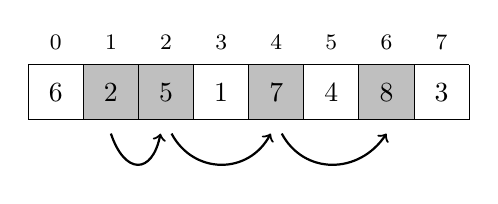
\begin{tikzpicture}[scale=0.7]
\fill[color=lightgray] (1,0) rectangle (2,1);
\fill[color=lightgray] (2,0) rectangle (3,1);
\fill[color=lightgray] (4,0) rectangle (5,1);
\fill[color=lightgray] (6,0) rectangle (7,1);
\draw (0,0) grid (8,1);
\node at (0.5,0.5) {$6$};
\node at (1.5,0.5) {$2$};
\node at (2.5,0.5) {$5$};
\node at (3.5,0.5) {$1$};
\node at (4.5,0.5) {$7$};
\node at (5.5,0.5) {$4$};
\node at (6.5,0.5) {$8$};
\node at (7.5,0.5) {$3$};

\draw[thick,->] (1.5,-0.25) .. controls (1.75,-1.00) and (2.25,-1.00) .. (2.4,-0.25);
\draw[thick,->] (2.6,-0.25) .. controls (3.0,-1.00) and (4.0,-1.00) .. (4.4,-0.25);
\draw[thick,->] (4.6,-0.25) .. controls (5.0,-1.00) and (6.0,-1.00) .. (6.5,-0.25);

\footnotesize
\node at (0.5,1.4) {$0$};
\node at (1.5,1.4) {$1$};
\node at (2.5,1.4) {$2$};
\node at (3.5,1.4) {$3$};
\node at (4.5,1.4) {$4$};
\node at (5.5,1.4) {$5$};
\node at (6.5,1.4) {$6$};
\node at (7.5,1.4) {$7$};
\end{tikzpicture}
\end{center}

$\texttt{length}(k)$ を$k$文字目まで見た時の
LISとしましょう。
したがって$0 \le k \le n-1$
となる$\texttt{length}(k)$の値をすべて計算すれば,
最も長く増加 する部分列の長さが求められます。
例えば,上の配列に対する関数の値は 以下の通りである.

\[
\begin{array}{lcl}
\texttt{length}(0) & = & 1 \\
\texttt{length}(1) & = & 1 \\
\texttt{length}(2) & = & 2 \\
\texttt{length}(3) & = & 1 \\
\texttt{length}(4) & = & 3 \\
\texttt{length}(5) & = & 2 \\
\texttt{length}(6) & = & 4 \\
\texttt{length}(7) & = & 2 \\
\end{array}
\]

例えば,$\texttt{length}(6)=4$は
位置6で終わる最も長い増加部分配列が4要素で構成されることを示します。

$\texttt{length}(k)$の値を計算するには、
$\texttt{array}[i]<\texttt{array}[k]$であって、
$\texttt{length}(i)$ができるだけ大きくなる位置$i < k$を見つければよいです。
そうすると、$\texttt{length}(k)=\texttt{length}(i)+1$となり、
これが$\texttt{array}[k]$を部分配列に追加する最適な方法であるとわかります。
しかし,そのような位置$i$がない場合には$\texttt{length}(k)=1$となり
部分配列には$\texttt{array}[k]$しか含まれないことになります.

関数のすべての値はその小さい値から計算できるので、
動的計画法を使うことができる。次のコードでは、関数の値は配列$\texttt{length}$に格納されます。

\begin{lstlisting}
for (int k = 0; k < n; k++) {
    length[k] = 1;
    for (int i = 0; i < k; i++) {
        if (array[i] < array[k]) {
            length[k] = max(length[k],length[i]+1);
        }
    }
}
\end{lstlisting}

このコードは2つのネストされたループで構成されているため$O(n^2)$で動作します。
しかし、動的計画法の計算をより効率的に $O(n \log n)$時間で実装することも可能です。
あなたはこの方法を見つけることができますか?

\section{グリッド上のパス - Paths in a grid}

次の問題は、$n \times n$ のグリッドの左上隅から右下隅まで、
下と右にしか移動しないような経路を見つける問題です。
各マスには正の整数が含まれており、
経路に沿った値の合計ができるだけ大きくなるように経路を構成したいとします。

下図は、格子状のマスの例とその最適経路を示したものです。
\begin{center}
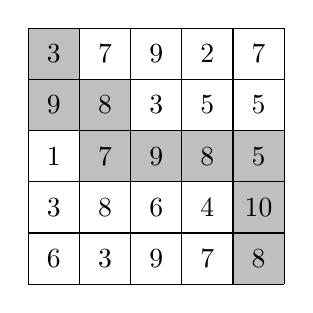
\begin{tikzpicture}[scale=.65]
  \begin{scope}
    \fill [color=lightgray] (0, 9) rectangle (1, 8);
    \fill [color=lightgray] (0, 8) rectangle (1, 7);
    \fill [color=lightgray] (1, 8) rectangle (2, 7);
    \fill [color=lightgray] (1, 7) rectangle (2, 6);
    \fill [color=lightgray] (2, 7) rectangle (3, 6);
    \fill [color=lightgray] (3, 7) rectangle (4, 6);
    \fill [color=lightgray] (4, 7) rectangle (5, 6);
    \fill [color=lightgray] (4, 6) rectangle (5, 5);
    \fill [color=lightgray] (4, 5) rectangle (5, 4);
    \draw (0, 4) grid (5, 9);
    \node at (0.5,8.5) {3};
    \node at (1.5,8.5) {7};
    \node at (2.5,8.5) {9};
    \node at (3.5,8.5) {2};
    \node at (4.5,8.5) {7};
    \node at (0.5,7.5) {9};
    \node at (1.5,7.5) {8};
    \node at (2.5,7.5) {3};
    \node at (3.5,7.5) {5};
    \node at (4.5,7.5) {5};
    \node at (0.5,6.5) {1};
    \node at (1.5,6.5) {7};
    \node at (2.5,6.5) {9};
    \node at (3.5,6.5) {8};
    \node at (4.5,6.5) {5};
    \node at (0.5,5.5) {3};
    \node at (1.5,5.5) {8};
    \node at (2.5,5.5) {6};
    \node at (3.5,5.5) {4};
    \node at (4.5,5.5) {10};
    \node at (0.5,4.5) {6};
    \node at (1.5,4.5) {3};
    \node at (2.5,4.5) {9};
    \node at (3.5,4.5) {7};
    \node at (4.5,4.5) {8};
  \end{scope}
\end{tikzpicture}
\end{center}
パス上の値の合計は67であり、これは左上隅から右下隅までのパスで可能な最大の合計である。

格子の行と列には1から$n$までの番号が振られ、
$\texttt{value}[y][x]$  はマス$(y,x)$ の値に等しいとしましょう。
$\texttt{sum}(y,x)$ は左上隅から$(y,x)$までの経路上の最大和を表すとします。
ここで、$\texttt{sum}(n,n)$は左上隅から右下隅までの最大和を表します。
例えば、上の格子では、$\texttt{sum}(5,5)=67$であると言えます。

この問題は以下のように再帰的に総和を計算することができます。

\[ \texttt{sum}(y,x) = \max(\texttt{sum}(y,x-1),\texttt{sum}(y-1,x))+\texttt{value}[y][x]\]

何故なら、マス $(y,x)$への道は次のように$(y-1,x)$か $(y,x-1)$からくるという観察に基づきます。

\begin{center}
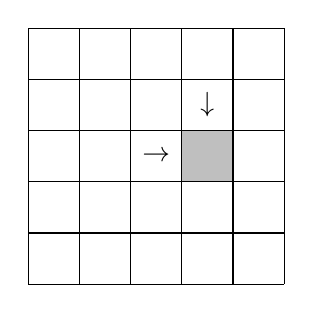
\begin{tikzpicture}[scale=.65]
  \begin{scope}
    \fill [color=lightgray] (3, 7) rectangle (4, 6);
    \draw (0, 4) grid (5, 9);
    
    \node at (2.5,6.5) {$\rightarrow$};
    \node at (3.5,7.5) {$\downarrow$};
    
  \end{scope}
\end{tikzpicture}
\end{center}

つまり、この式は和を最大化する方向を選択します。
$y=0$ か $x=0$なら その方向からの入力は$\texttt{sum}(y,x)=0$として計算します。

関数 \texttt{sum}は 2 つのパラメータを持つので動的計画法配列も2次元になります。

\begin{lstlisting}
int sum[N][N];
\end{lstlisting}
を次のように計算していきます。
\begin{lstlisting}
for (int y = 1; y <= n; y++) {
    for (int x = 1; x <= n; x++) {
        sum[y][x] = max(sum[y][x-1],sum[y-1][x])+value[y][x];
    }
}
\end{lstlisting}

これは$O(n^2)$で計算可能です。

\section{ナップザック問題 - Knapsack problems}

\index{ナップザック問題 - knapsack}

\key{knapsack - ナップザック問題 }とは、
集合が与えられ、ある性質を持った部分集合を見つけなければならない問題のことです。
ナップザック問題は多くの場合動的計画法を用いて解くことができます。

重みのリスト$[w_1,w_2,\ldots,w_n]$が与えられたとき、
その重みを使って構成できるすべての和を決定することなどが例に挙げられます。
例えば、重みが$[1,3,3,5]$の場合、以下の和が可能です。

\begin{center}
\begin{tabular}{rrrrrrrrrrrrr}
 0 & 1 & 2 & 3 & 4 & 5 & 6 & 7 & 8 & 9 & 10 & 11 & 12 \\
\hline
 X & X & & X & X & X & X & X & X & X & & X & X \\
\end{tabular}
\end{center}

この場合、2と10を除く$0 \ldots 12$の間のすべての和が実現可能であることを意味します。
例えば、和7は、重み$[1,3,3]$を選んで実現可能です。

この問題を解くために、最初の$k$個の重みだけを用いて和を構成する部分問題に注目しましょう。
最初の$k$個の重みを使って和$x$を構成できる場合は
$\texttt{possible}(x,k)=\textrm{true}、
そうでない場合は
$\texttt{possible}(x,k)=\textrm{false}とします。
この関数の値は以下のように再帰的に計算することができます。
\[ \texttt{possible}(x,k) = \texttt{possible}(x-w_k,k-1) \lor \texttt{possible}(x,k-1) \]
この式は、和に重み$w_k$を使うか使わないかのどちらかを選ぶことができることに基づいています。
$w_k$を使う場合、
残りのタスクは最初の$k - 1$個の重みを使って 和$x-w_k$ を形成することであり、
$w_k$を使わない場合、残りのタスクは最初の$k - 1$個の重みを使って和$x$を形成することになります。

また、初期状態として
\begin{equation*}
    \texttt{possible}(x,0) = \begin{cases}
               \textrm{true}    & x = 0\\
               \textrm{false}   & x \neq 0 \\
           \end{cases}
\end{equation*}
が与えられます。というのは、重みがない場合は、和は0にしかならないからです。

次の表は、重み $[1,3,3,5]$  に対する関数のすべての値を示しています(記号 ''X''は真の値を示す)。
\begin{center}
\begin{tabular}{r|rrrrrrrrrrrrr}
$k \backslash x$ & 0 & 1 & 2 & 3 & 4 & 5 & 6 & 7 & 8 & 9 & 10 & 11 & 12 \\
\hline
 0 & X & \\
 1 & X & X \\
 2 & X & X & & X & X \\
 3 & X & X & & X & X & & X & X \\
 4 & X & X & & X & X & X & X & X & X & X & & X & X \\
\end{tabular}
\end{center}

これらの値を計算した後、$\texttt{possible}(x,n)$は、
すべての重みを使って和$x$を構 成できるかどうかを教えてくれる。

$W$は重みの総和を表すとする。以下の$O(nW)$ 時間の動的計画法が再帰関数に相当します。
\begin{lstlisting}
possible[0][0] = true;
for (int k = 1; k <= n; k++) {
    for (int x = 0; x <= W; x++) {
        if (x-w[k] >= 0) possible[x][k] |= possible[x-w[k]][k-1];
        possible[x][k] |= possible[x][k-1];
    }
}
\end{lstlisting}

さて、ここでは,和が$x$の部分集合を構成できるかどうかを示す1次元配列
$\texttt{possible}[x]$のみを用いるよりよい実装を示しましょう。
この配列は,新しい重みごとに右から左へと更新します。

\begin{lstlisting}
possible[0] = true;
for (int k = 1; k <= n; k++) {
    for (int x = W; x >= 0; x--) {
        if (possible[x]) possible[x+w[k]] = true;
    }
}
\end{lstlisting}

なお、ここで紹介した一般的な考え方は、多くのナップザック問題で利用することができます
例えば、重みと価値を持つオブジェクトが与えられた場合に、各重み和について部分集合の最大の価値を決定することができます。

\section{編集距離 - Edit distance}

\index{編集距離 - edit distance}
\index{レーベンシュタイン距離 - Levenshtein distance}

\key{編集距離 - edit distance} あるいは \key{レーベンシュタイン距離 - Levenshtein distance}
\footnote{The distance
is named after V. I. Levenshtein who studied it in connection with binary codes \cite{lev66}.}
とは、ある文字列を別の文字列に変換するために必要な編集操作の最小回数のことである。
編集操作とは以下の通りである。

\begin{itemize}
\item 挿入 (e.g. \texttt{ABC} $\rightarrow$ \texttt{ABCA})
\item 削除 (e.g. \texttt{ABC} $\rightarrow$ \texttt{AC})
\item 変更 (e.g. \texttt{ABC} $\rightarrow$ \texttt{ADC})
\end{itemize}

例えば、\texttt{LOVE} と \texttt{MOVIE} の編集距離は2です。
これは、まず\texttt{LOVE}$\rightarrow$ \texttt{MOVE}(変更)の操作を行い、
次に\texttt{MOVE}$\rightarrow$ \texttt{MOVIE}(挿入)の操作で一致させられます。
1つの操作だけでは不十分であることが明らかであるため可能な限り少ない操作回数であることは明らかでしょう。

長さ$n$の文字列\texttt{x}と長さ$m$の文字列\texttt{y} が与えられたときの
\texttt{x}と\texttt{y} の編集距離を計算します。
この問題を解決するために、接頭辞$\texttt{x}[0 \ldots a]$ と $\texttt{y}[0 \ldots b]$
の編集距離を与える関数distance(a、b)を定義します。
この関数を用いると,\texttt{x} と\texttt{y}  の編集距離は
$\texttt{distance}(n-1,m-1)$に等しくなる.

\texttt{distance}は次のように計算することができます。
\begin{equation*}
\begin{split}
\texttt{distance}(a,b) = \min(& \texttt{distance}(a,b-1)+1, \\
                           & \texttt{distance}(a-1,b)+1, \\
                           & \texttt{distance}(a-1,b-1)+\texttt{cost}(a,b)).
\end{split}
\end{equation*}
ここで、$\texttt{x}[a]=\texttt{y}[b]$ならば $\texttt{cost}(a,b)=0$、
そうでなければ $\texttt{cost}(a,b)=1$とします。
この式では、文字列\texttt{x}の編集方法として、次のようなものを考えている。

\begin{itemize}
\item $\texttt{distance}(a,b-1)$: \texttt{x}の最後に文字の挿入を行う
\item $\texttt{distance}(a-1,b)$: \texttt{x}の文字を最後を削除する
\item $\texttt{distance}(a-1,b-1)$: \texttt{x}の最後の文字が一致あるいは変更する
\end{itemize}
最初の2つのケースでは、1つの編集操作(挿入または削除)が必要です。
最後の場合、$\texttt{x}[a]=\texttt{y}[b]$であれば、
編集なしで最後の文字をマッチングさせることができ、
そうでなければ、1つの編集操作(modify)が必要になります。
次の表は、例の場合の\texttt{distance}の値を示したものです。

\begin{center}
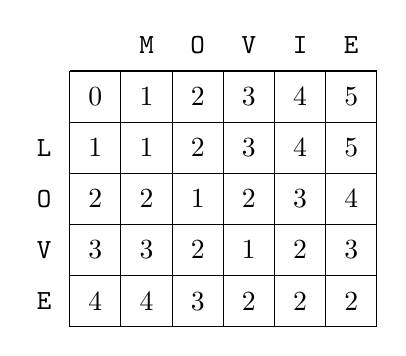
\begin{tikzpicture}[scale=.65]
  \begin{scope}
    %\fill [color=lightgray] (5, -3) rectangle (6, -4);
    \draw (1, -1) grid (7, -6);
    
    \node at (0.5,-2.5) {\texttt{L}};
    \node at (0.5,-3.5) {\texttt{O}};
    \node at (0.5,-4.5) {\texttt{V}};
    \node at (0.5,-5.5) {\texttt{E}};

    \node at (2.5,-0.5) {\texttt{M}};
    \node at (3.5,-0.5) {\texttt{O}};
    \node at (4.5,-0.5) {\texttt{V}};
    \node at (5.5,-0.5) {\texttt{I}};
    \node at (6.5,-0.5) {\texttt{E}};

    \node at (1.5,-1.5) {$0$};
    \node at (1.5,-2.5) {$1$};
    \node at (1.5,-3.5) {$2$};
    \node at (1.5,-4.5) {$3$};
    \node at (1.5,-5.5) {$4$};
    \node at (2.5,-1.5) {$1$};
    \node at (2.5,-2.5) {$1$};
    \node at (2.5,-3.5) {$2$};
    \node at (2.5,-4.5) {$3$};
    \node at (2.5,-5.5) {$4$};
    \node at (3.5,-1.5) {$2$};
    \node at (3.5,-2.5) {$2$};
    \node at (3.5,-3.5) {$1$};
    \node at (3.5,-4.5) {$2$};
    \node at (3.5,-5.5) {$3$};
    \node at (4.5,-1.5) {$3$};
    \node at (4.5,-2.5) {$3$};
    \node at (4.5,-3.5) {$2$};
    \node at (4.5,-4.5) {$1$};
    \node at (4.5,-5.5) {$2$};
    \node at (5.5,-1.5) {$4$};
    \node at (5.5,-2.5) {$4$};
    \node at (5.5,-3.5) {$3$};
    \node at (5.5,-4.5) {$2$};
    \node at (5.5,-5.5) {$2$};
    \node at (6.5,-1.5) {$5$};
    \node at (6.5,-2.5) {$5$};
    \node at (6.5,-3.5) {$4$};
    \node at (6.5,-4.5) {$3$};
    \node at (6.5,-5.5) {$2$};
  \end{scope}
\end{tikzpicture}
\end{center}

表の右下には、\texttt{LOVE}と\texttt{MOVIE}の編集距離が2であることが示されています。
この表は最短の編集操作の順序を構築する方法も示されています。この場合の経路は次のようになります。
\begin{center}
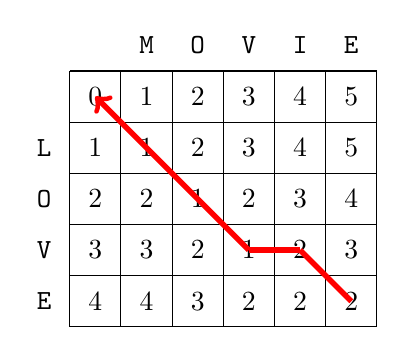
\begin{tikzpicture}[scale=.65]
  \begin{scope}
    \draw (1, -1) grid (7, -6);
    
    \node at (0.5,-2.5) {\texttt{L}};
    \node at (0.5,-3.5) {\texttt{O}};
    \node at (0.5,-4.5) {\texttt{V}};
    \node at (0.5,-5.5) {\texttt{E}};

    \node at (2.5,-0.5) {\texttt{M}};
    \node at (3.5,-0.5) {\texttt{O}};
    \node at (4.5,-0.5) {\texttt{V}};
    \node at (5.5,-0.5) {\texttt{I}};
    \node at (6.5,-0.5) {\texttt{E}};

    \node at (1.5,-1.5) {$0$};
    \node at (1.5,-2.5) {$1$};
    \node at (1.5,-3.5) {$2$};
    \node at (1.5,-4.5) {$3$};
    \node at (1.5,-5.5) {$4$};
    \node at (2.5,-1.5) {$1$};
    \node at (2.5,-2.5) {$1$};
    \node at (2.5,-3.5) {$2$};
    \node at (2.5,-4.5) {$3$};
    \node at (2.5,-5.5) {$4$};
    \node at (3.5,-1.5) {$2$};
    \node at (3.5,-2.5) {$2$};
    \node at (3.5,-3.5) {$1$};
    \node at (3.5,-4.5) {$2$};
    \node at (3.5,-5.5) {$3$};
    \node at (4.5,-1.5) {$3$};
    \node at (4.5,-2.5) {$3$};
    \node at (4.5,-3.5) {$2$};
    \node at (4.5,-4.5) {$1$};
    \node at (4.5,-5.5) {$2$};
    \node at (5.5,-1.5) {$4$};
    \node at (5.5,-2.5) {$4$};
    \node at (5.5,-3.5) {$3$};
    \node at (5.5,-4.5) {$2$};
    \node at (5.5,-5.5) {$2$};
    \node at (6.5,-1.5) {$5$};
    \node at (6.5,-2.5) {$5$};
    \node at (6.5,-3.5) {$4$};
    \node at (6.5,-4.5) {$3$};
    \node at (6.5,-5.5) {$2$};

    \path[draw=red,thick,-,line width=2pt] (6.5,-5.5) -- (5.5,-4.5);
    \path[draw=red,thick,-,line width=2pt] (5.5,-4.5) -- (4.5,-4.5);
    \path[draw=red,thick,->,line width=2pt] (4.5,-4.5) -- (1.5,-1.5);
  \end{scope}
\end{tikzpicture}
\end{center}

\texttt{LOVE} and \texttt{MOVIE}は最後の文字が等しいので、
両者の編集距離は\texttt{LOV} と \texttt{MOVI}の編集距離と等しくなる。
\texttt{MOVI}から\texttt{I}という文字を削除するには、
1回の編集操作で可能である。
したがって、編集距離は\texttt{LOV}と\texttt{MOV}の間の編集距離より1大きいといったように読み取ります。

\section{タイルの数え上げ - Counting tilings}

動的計画法の計算の過程は、単に固定された数の組み合わせよりも複雑な場合があります。
例えば、$1 \times 2$ と $2 \times 1$のタイルを使って、
$n \times m$ の格子を何通り埋めることができるかを計算する問題を考えてみよう。
例えば、$4 \times 7$ グリッドの有効な解は以下の通りです。

\begin{center}
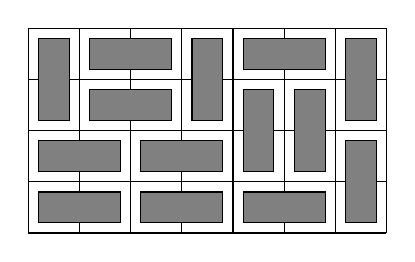
\begin{tikzpicture}[scale=.65]
    \draw (0,0) grid (7,4);
    \draw[fill=gray] (0+0.2,0+0.2) rectangle (2-0.2,1-0.2);
    \draw[fill=gray] (2+0.2,0+0.2) rectangle (4-0.2,1-0.2);
    \draw[fill=gray] (4+0.2,0+0.2) rectangle (6-0.2,1-0.2);
    \draw[fill=gray] (0+0.2,1+0.2) rectangle (2-0.2,2-0.2);
    \draw[fill=gray] (2+0.2,1+0.2) rectangle (4-0.2,2-0.2);
    \draw[fill=gray] (1+0.2,2+0.2) rectangle (3-0.2,3-0.2);
    \draw[fill=gray] (1+0.2,3+0.2) rectangle (3-0.2,4-0.2);
    \draw[fill=gray] (4+0.2,3+0.2) rectangle (6-0.2,4-0.2);

    \draw[fill=gray] (0+0.2,2+0.2) rectangle (1-0.2,4-0.2);
    \draw[fill=gray] (3+0.2,2+0.2) rectangle (4-0.2,4-0.2);
    \draw[fill=gray] (6+0.2,2+0.2) rectangle (7-0.2,4-0.2);
    \draw[fill=gray] (4+0.2,1+0.2) rectangle (5-0.2,3-0.2);
    \draw[fill=gray] (5+0.2,1+0.2) rectangle (6-0.2,3-0.2);
    \draw[fill=gray] (6+0.2,0+0.2) rectangle (7-0.2,2-0.2);

\end{tikzpicture}
\end{center}
この場合、総解答数は781となります。

この問題は動的計画法を用いて、グリッドの行を1つずつ調べていくことで解くことができます。
解の各行は、集合 $\{\sqcap, \sqcup, \sqsubset, \sqsupset \}$から $m$個の
文字を含む文字列として表すことができます。
例えば、上の解答は4つの行からなり、それらは 以下の文字列に対応する。

\begin{itemize}
\item
$\sqcap \sqsubset \sqsupset \sqcap \sqsubset \sqsupset \sqcap$
\item
$\sqcup \sqsubset \sqsupset \sqcup \sqcap \sqcap \sqcup$
\item
$\sqsubset \sqsupset \sqsubset \sqsupset \sqcup \sqcup \sqcap$ 
\item
$\sqsubset \sqsupset \sqsubset \sqsupset \sqsubset \sqsupset \sqcup$
\end{itemize}

$\texttt{count}(k,x)$は、文字列$x$が$k$行目に対応するようなグリッド
の$1 \ldots k$行目の解を構成する方法の数を表すとしましょう。
ある行の状態は前の行の状態によってのみ制約されるので動的計画法を使用することができます。

1行目に$\sqcup$という文字がなく、
n行目に$\sqcap$という文字がなく、
かつ連続するすべての行が対応を持っていれば、
解は成立する。例えば$\sqcup \sqsubset \sqsupset \sqcup \sqcap \sqcap \sqcup$ と
$\sqsubset \sqsupset \sqsubset \sqsupset \sqcup \sqcup \sqcap$ の行は対応があり、
$\sqcap \sqsubset \sqsupset \sqcap \sqsubset \sqsupset \sqcap$ と
$\sqsubset \sqsupset \sqsubset \sqsupset \sqsubset \sqsupset \sqcup$の行は対応がない。

1行は$m$個の文字からなり、各文字には4つの選択肢があるので、異なる行の数は最大でも$4^m$です。
したがって、各行について$O(4^m)$ 個の可能な 状態を調べ、
それぞれの状態について、前の行について$O(4^m)$  個の可能な状態があるので、
解法の時間計算量は$O(n 4^{2m})$となります。
係数$4^{2m}$が時間計算量を支配するので、
短い方の辺の長さが$m$になるようにグリッドを回転させるのがよいでしょう。

行をよりコンパクトに表現することで、より効率的に解を得ることができます。
前の行のどの列が縦長のタイルの上側の正方形を含むかが分かればよいと分かったので、
$\sqcap$ と $\Box$だけで表現ができます。
$\Box$は、$\sqcup$, $\sqsubset$ , $\sqsupset$.の組み合わせである。
この表現を用いると、$2^m$個の行を表現できるため、
$O(n 2^{2m})$で良いです。

最後に、タイリングを求めるためには驚くべき公式があります。\footnote{Surprisingly,
this formula was discovered in 1961 by two research teams \cite{kas61,tem61}
that worked independently.}
\[ \prod_{a=1}^{\lceil n/2 \rceil} \prod_{b=1}^{\lceil m/2 \rceil} 4 \cdot (\cos^2 \frac{\pi a}{n + 1} + \cos^2 \frac{\pi b}{m+1})\]
この式は、タイリングの数を$O(nm)$で計算するため、
非常に効率的です。ただし、答えが実数の積であるため、この式を使う場合は
中間結果をいかに正確に保存するかが問題となります。


